\chapter{Inverse Kinematics in the Unity Engine} 
The demo application written for the purpose of this paper includes two separate
use cases of skeletal animation using inverse kinematics in the Unity engine.
The first example is that of a four legged spider which uses IK as a means to
more naturally adjust its limbs to the terrain it moves around upon. The second
example is the application of inverse kinematics to an animation sequence of
a human character pressing multiple buttons in succession. The use of inverse
kinematics allows the character to adjust its animation to hit all the buttons
without the need for a baked animation targeted towards each button, as well as
dynamically adjust the order of the buttons to be hit. Although there are two
separate use cases demonstrated in this application, both use the same
implementation of the FABRIK algorithm. 


\section{FABRIK implementation}
This implementation of the FABRIK algorithm is based on the paper written by the
author of the Unity engine FABRIK implementation \cite{Aristidou2011}. For the
purposes of this application, the basic algorithm is implemented without many
additional constraints and limitation on the chain's degrees of freedom. The one
constraint added on to this implementation is that of pole targets which will be
further explained when discussing the code behind them.

The script which implements the algorithm in this project takes in a few
parameters required to set up the mechanism which are shown in Figure
\ref{fig:params}. First and foremost, the root and leaf nodes must be provided
in order to define the kinematic chain which is to be manipulated. The next
object which the script must have knowledge of is the target transform which the
end effector will attempt to move to. The script must also have a tolerance
parameter which dictates how close the end effector must be to the target for
the position to be considered as solved. All the aforementioned parameters are
required for the script to function. Optionally, a pole target object may be
passed in if the use case requires it to function in a desired manner. 

\begin{figure}
    \centering
    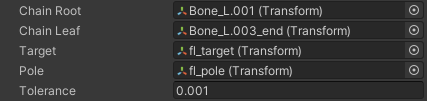
\includegraphics{grafika/parametry_ik.png}
    \caption{FABRIK script parameters}
    \label{fig:params}
\end{figure}

The first case which the algorithm must cover is if the distance from the root
to the target object is greater than the sum of distances between each adjacent
bone transform in the defined kinematic chain. In this case, the target is out
of reach. Given that the bones in a skeleton are expected to keep a fixed
length, the end effector will not be able to reach the target, and instead the
kinematic chain straightens and extends in the direction of the target. There is
no need to continue with the iterative portion of the algorithm.

A minor optimization in the implementation is the use of square magnitudes when
comparing distances to avoid the calculation of square roots, thus reducing the
computational costs.

% \begin{lstlisting}[basicstyle=\footnotesize, numbers=none,frame=single, caption={Target out of
% reach},captionpos=b, label=stretch, language={[Sharp]c}]
% void LateUpdate() 
% {
%     float distRootToTargetSqr = (
%         target.position - chainRoot.position
%     ).sqrMagnitude;
%     if (distRootToTargetSqr > totalDistance * totalDistance)
%     {
%         StretchToTarget();
%     }
%     ...
% }

% void StretchToTarget()
% {
%     for (var i = 0; i < chainLen; i++)
%     {
%         float jointDistToTarget = (
%             target.position - tempPositions[i]
%         ).magnitude;
%         var lambda = jointDistances[i] / jointDistToTarget;

%         tempPositions[i + 1] =
%             (1 - lambda) * tempPositions[i] + lambda * target.position;
%     }
% }
% \end{lstlisting}

The scenario where the target is within the reach of the kinematic chain
utilizes an iterative forward and backward component after which the algorithm is
named. Before each iteration, the positions of the joint transforms are copied.
All operations and calculations are performed on these copied transforms and at
the end of the full pass, the new positions are then copied back to the
kinematic chain. It is also important to note that the modification of the
transforms is done in Unity's \textit{LateUpdate} function. When using a mix of
inverse kinematics and baked animation, the object to which the IK script is
attached will have Unity's built-in \textit{Animator} component attached. If the
custom IK script were to update joint transforms in the \textit{Update} method,
then their attributes may be overwritten by the \textit{Animator} component. 

The forward pass of the algorithm iterates through the chain starting from the
end effector and ending at the root. At the start, the end effector's position
is set to be equal to the position of the target. A straight line can then be
imagined to exist between the end effector and the following node. This
neighbor's position is then interpolated along the line so that the original
distance between the two nodes is kept the same. The same operation is performed
for each pair of neighboring nodes throughout the pass. 

% \begin{lstlisting}[basicstyle=\footnotesize, numbers=none,frame=single,
% caption={Forward pass},captionpos=b, label=forwards, language={[Sharp]c}]
% void ForwardReachingPass()
% {
%     tempPositions[chainLen] = target.position;
%     for (var i = chainLen - 1; i >= 0; i--)
%     {
%         var dist = (tempPositions[i + 1] - tempPositions[i]).magnitude;
%         var lambda = jointDistances[i] / dist;
%         tempPositions[i] =
%             (1 - lambda) * tempPositions[i + 1]
%             + lambda * tempPositions[i];
%     }
% }
% \end{lstlisting}

When the forward pass is complete, the root node is displaced from its original
position. This is undesired, as the root's node position should not be affected
by the algorithm. To remedy this, the next step is to repeat the forwards pass,
but this time in reverse. The root node's position is set equal to what it was
at the beginning of the frame. The next node is then interpolated between its
current position and the root to keep the initial bone length. As with the
forward pass, this is repeated for each subsequent pair of nodes. 

% \begin{lstlisting}[basicstyle=\footnotesize, numbers=none,frame=single,
% caption={Backward pass},captionpos=b, label=backwards, language={[Sharp]c}]
% void BackwardReachingPass()
% {
%     tempPositions[0] = chainRoot.position;
%     for (var i = 0; i < chainLen; i++)
%     {
%         var dist = (tempPositions[i + 1] - tempPositions[i]).magnitude;
%         var lambda = jointDistances[i] / dist;
%         tempPositions[i + 1] =
%             (1 - lambda) * tempPositions[i]
%             + lambda * tempPositions[i + 1];
%     }
% }
% \end{lstlisting}

These two steps are repeated together until the end effector is within
a threshold distance of the target. The FABRIK algorithm is a heuristic
algorithm, and as such it does not lead to an exact result. Instead, it aims to
approximate the correct solution and solves the problem in a less complex and
more optimized way. Again, the square distances are used to avoid the
calculation of square roots. 

% \begin{lstlisting}[basicstyle=\footnotesize, numbers=none,frame=single,
% caption={FABRIK Loop},captionpos=b, label=loop, language={[Sharp]c}]
% void LateUpdate()
% {
%     ...
%     else
%     {
%         var distEffectorToTargetSqr = (
%             tempPositions[chainLen] - target.position
%         ).sqrMagnitude;
%         while (distEffectorToTargetSqr > tolerance * tolerance)
%         {
%             ForwardReachingPass();
%             BackwardReachingPass();

%             distEffectorToTargetSqr = (
%                 tempPositions[chainLen] - target.position
%             ).sqrMagnitude;
%         }
%         ...
%     }

%     ApplyTempPositions();
% }
% \end{lstlisting}

While the basic FABRIK algorithm allows a kinematic chain adjust so that the end
effector reaches a defined target, the lack of control over this process can
lead to unnatural poses in certain use cases, defeating the purpose of the
procedural animations which are designed to produce a more natural effect. In
order to achieve a higher degree of control in one of the use cases described in
the following section, pole target constraints were implemented as an optional
supplement to the existing algorithm. This approach to the pole target algorithm
is inspired by a video demonstrating this concept CITE.

The pole algorithm acts on every joint in a given kinematic chain excluding the
root and the target which already have positions which are defined exactly. For
each of the iterated joints \textit{p[i]}, calculations must take into account
the positions of their preceding joint \textit{p[i-1]} and succeeding joint
\textit{p[i+1]}. A plane is constructed at the position the \textit{p[i-1]},
with a normal vector which points from \textit{p[i-1]} to \textit{p[i+1]}. Both
the pole and the currently manipulated joint are then projected onto the plane
(Figure \ref{fig:pole_start}) using Unity plane's \textit{ClosestPointOnPlane}
method. The \textit{Vector3.SignedAngle} method then allows an angle to be found
between both projections by passing the plane's normal vector as the angle axis
(Figure \ref{fig:pole_projection}). Finally, the current joint's desired
position is calculated by rotating the vector between it and \textit{p[i-1]}
around the plane's normal by the obtained angle, using the
\textit{Quaternion.AngleAxis} method. This can be imagined as lining up the
joint so that its planar projection exists on the line between the origin of the
plane and the pole target's planar projection (Figure \ref{fig:pole_end}). The
joint keeps its relation to its preceding and succeeding joints (the angle
between vectors pointing from the joint to both surrounding joints is the same),
but it is rotated in order to be positioned as close to the pole target as
possible.

\begin{figure}[!h]
    \centering
    \captionsetup{justification=centering}
    \begin{subfigure}{\textwidth}
        \centering
        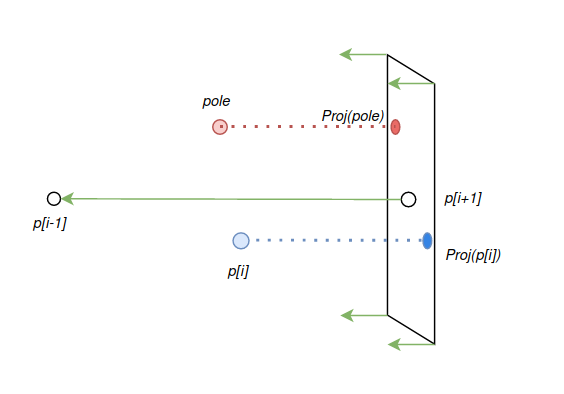
\includegraphics[width=0.6\linewidth]{grafika/pole_start.png}
        \subcaption{The initial setup where a plane is constructed with the
        vector from \textit{p[i+1]} to \textit{p[i-1]} as the normal. Both the
        current joint \textit{p[i]} and the pole target are projected onto the
        plane}
        \label{fig:pole_start}
    \end{subfigure}
    \begin{subfigure}{\textwidth}
        \centering
        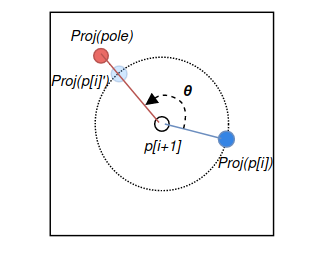
\includegraphics[width=0.4\linewidth]{grafika/pole_projection.png}
        \subcaption{A view of the plane and the angle between the
            projections which dictates the new position of the joint
            \textit{p[i]}}
        \label{fig:pole_projection}
    \end{subfigure}
    \begin{subfigure}{\textwidth}
        \centering
        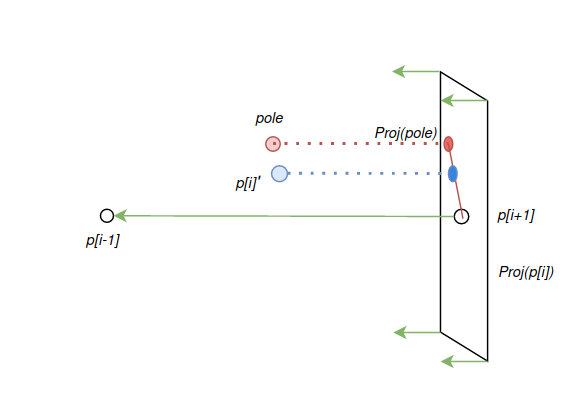
\includegraphics[width=0.6\linewidth]{grafika/pole_end.png}
        \subcaption{The final position of the joint as a result of the pole
        target mechanism}
        \label{fig:pole_end}
    \end{subfigure}
    \caption{A diagram showing the concept behind the implemented pole target
    mechanism}
    \label{fig:pole_diagram}
\end{figure}


FIGURE

\section{Spider Movement}
The first use case for inverse kinematics in the demo application is that of
a four legged spider. The algorithm is used to adjust the creature's limbs to
uneven terrain, leading to a much more natural and realistic movement. The IK
version of the spider does not have an Animator component, and the whole of the
animation and movement of the spider and its legs is done procedurally.
\subsection{Project Setup}
Each one of the spiders legs is treated as a separate kinematic chain. The
spider prefab consists of a container which holds the spider object itself, set
of empty objects to which the four IK scripts are attached for the purpose of
easy yet separated access. The prefab also contains sets of ray casts and
targets. The ray casts serve to scan the surface of the terrain under the
spider, and mark the targets to which each leg should move.

Ray casts are dispatched from above the spiders legs, and aim in the creatures
local negative Y axis. This ensures that no matter what orientation the spider
finds itself in, the rays are always pointing at the surface which it is
standing on. Masks are applied to the rays, making sure that only terrain
objects are taken into account, while the creature's body itself is not. The ray
cast hit point positions are then applied to each leg's respective target
object. These targets serve as markers for the limbs end effectors. 

\subsection{Scripts}
With the project set up in this manner, scripts must now be added on to make the
scene functional. A script is required for the main movement of the spider, the
ray cast logic, and the mechanism which controls the ik targets.

\subsubsection{Ray casts}
The ray cast objects contain a script component which dispatches the rays and
sets the appropriate target positions. First, a mask must be established, which
will then be passed into the ray cast operation. This is required so that only
terrain is counted as a valid hit. The lack of such a mask may result in
unexpected behavior, such as targets being set on the spider's body itself. The
ray cast object is then created, shooting in the local negative Y axis
direction. This ensures that no matter the orientation of the creature, the rays
are sent towards the surface that the spider is standing on. The targets
controlling the spider's legs will not be updating their positions to the
ray cast hit points each frame, though their scripts must have knowledge of the
hit positions at any given time. Given this, a separate set of objects are set
to track the ray cast hit points each frame.

\subsubsection{Target Logic}
In order for the spider's movement to seem realistic, the targets controlling
each leg must adhere to a set of rules pertaining to their movement. As
mentioned in the ray cast section, the IK targets cannot simply be set to track
the ray cast hit points. The following is an outline of the rules specified for
the IK targets, which define if it should start moving towards its ray cast hit
target:
\begin{itemize}
    \item A target must be grounded to be eligible for a movement sequence.

    \item A target will only begin moving towards the ray cast hit point if the
        distance between them is above a specified threshold.

    \item A target is only allowed to begin moving towards the ray cast hit
        point if both legs on the opposite diagonal are grounded (See Figure
        \ref{fig:diagonals}).
\end{itemize}


\begin{figure}
    \centering
    \captionsetup{justification=centering}
    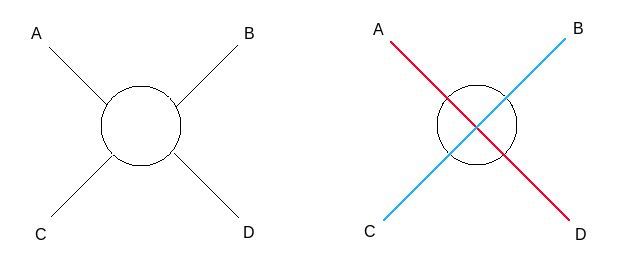
\includegraphics[width=0.8\textwidth]{grafika/diagonals.png}
    \caption{The diagonals referencing the spiders legs which are used when
    checking if a target is allowed to begin moving, where A and D are on an
opposite diagonal to B and C}
    \label{fig:diagonals}
\end{figure}

When a target satisfies all of these conditions, it makes note of the ray cast
hit's current position, which it will use for its upcoming movement sequence.
Once it begins moving, the \textit{Grounded} boolean is set to be false, so that
the other targets know whether they can begin moving or not.

The movement sequence itself is done using Unity's \textit{Vector3.MoveTowards}
method, which takes in a current position vector, a vector to move to, and the
maximum distance to move per frame, which can be used to control the movement
speed. This method allows the target to interpolate its position every frame.
The values fed into this method are simply the target's current position, the
ray cast hit target's position, which was recorded right before the beginning of
the movement sequence, and an arbitrary speed value, which is dependent on
\textit{Time.deltaTime} to avoid variations when the frame rate changes. The
only caveat is that in the first half of the movement, the destination vector's
height component is increased to achieve an arc-like movement. This produces the
effect of lifting the spider's leg.

\subsubsection{General Movement}
The main movement script for the IK spider implementation brings the whole
system together. It has three main objectives:

\begin{itemize}

    \item Calculate the rotation of the spider so that it's local up and forward
        vectors can be set accordingly.

    \item React to input by moving the main body of the spider along with the
        ray casts.

    \item Regulate the height of the spiders body above the ground.

\end{itemize}

The first objective - calculating the rotation of the spider - is what allows it
to scale walls and walk upside down on the ceiling. The rotation is determined
based on the limb positions at the beginning of each \textit{Update} call.
First, two vectors are constructed from the end effectors of both sets of
diagonally opposed legs. The local up vector of the spider is then calculated by
taking the cross product of these two vectors. This determines the orientation
of the spider's main body, and it also affects the direction that the four legs'
rays are cast. The local forward vector is then obtained from the cross product
between the newfound up vector and the spider's right vector. This new vector is
what will be used to determine the direction of movement when the spider
receives input from the user.

The second objective - reacting according to input - is quite simple once the
local directional axes are determined. When the script detects a non-zero value
on either the \textit{Horizontal} or \textit{Vertical} axis, it reacts
accordingly by moving the spider along with all the ray cast objects. The
\textit{Vertical} axis corresponds to the forward and backward movement of the
spider. The script reacts by simply moving the spider's main body along the
local forward axis mentioned previously. Additionally, the ray casting objects
are offset either forwards or backward depending on the direction of the
movement. This is done because the ray casts must be slightly ahead of the
default leg positions so that the legs end up moving in a natural manner.
The \textit{Horizontal} axis is responsible for rotating the spider about its
local up axis which allows the spider to turn around. 

Finally, the spider's height off of the surface must be regulated each frame.
The lack of a gravitational force acting on the body to keep it flush with the
ground, and the unconstrained rotational capability of the creature, means that
the distance between the spider and the surface it is walking on must be
procedurally kept in check. This is done with yet another ray cast which
originates from the center of the spider's body and points in the negative up
axis direction. If the distance to the hit point exceeds an acceptable range,
the body is moved towards said range, again using the
\textit{Vector3.MoveTowards} method to linearly interpolate the spiders position
and avoid excessive jerkiness which occurs with a frequent variation in height. 



\section{Human Animation Sequence}
The second example created to demonstrate the use of inverse kinematics for
skeletal animation in Unity is that of a human animation sequence which consists
of pressing multiple buttons in succession. While this may seem like a simple
animation to create in a tool like Blender, such an animation lacks the
adaptability needed for a game which has many differing button pressing
scenarios. The integration of IK into this kind of animation sequence adds the
ability to adjust to multiple amounts of buttons on a panel, different
configurations of button positions, various sequences of buttons to press, and
keep a consistent hand placement on the buttons without the need to force the
character to stand in one defined position. The example was not made solely
through the use of IK, and instead it uses a mix of baked animations for the
part of the animation which doesn't require variation, and IK for the part of
the animation which is subject to change.

\subsection{Project Setup}
A human model is exported from the MakeHuman software, imported into Blender for
animation, and then again exported and imported into the Unity engine. The scene
is set up with a group of buttons which are positioned on a wall. The buttons
themselves each have an \textit{EmptyObject} which will provide the transform
needed in order to aim the hand at the given button. The human character is
posted in front of this set up. An Animator component is attached to the human
model in order to make use of certain animations which were extracted from the
full button press animation created in Blender when importing the model into
Unity. Namely, the portions of the animation which consist of raising the hand
to the default pressing position and lowering it back down, are useful in the IK
version of this animation sequence. This is because these two animations are not
dependent on the amount of buttons on the wall, nor the position of the
character relative to the buttons.
\subsection{Scripts}
The whole logic around this animation sequence is done using one script. It must
take in a few public objects as parameters in order to work correctly (Figure
ref). Firstly, the hand's IK target must be passed in to enable the procedural
control of the model's position. The script must also have a reference to the
\textit{Rig} object to which the FABRIK script component is attached to. This is
needed in order to enable and disable the IK depending on the phase of the
animation sequence. When raising and lowering the hand, the baked animations are
used and the IK should be disabled. The next parameter is a list of transforms
for each button to which the IK target will move to in order to achieve the
effect of pressing a button. A couple of private variables are also declared to
make the script functional. These variables hold information such as references
to the animator and FABRIK script components, an idle variable which prevents
the character from starting a new animation sequence before finishing one that
was previously initiated, a value which determines the speed of the hand's
movement, and a list of integers which decide the sequence of buttons to be
pressed. One last variable holds the \textit{origin} position which is set to
the hand's position at the moment between the raising of the hand and the press
of a button. This transform is important because it is required in order for the
IK target to know where to return to after it is done pressing a given button. 

The main functionality of the script revolves around Unity's coroutines.
Coroutines enable a method to pause it's execution and then continue where it
left off on the next frame \cite{unity_coroutines}. This allows the method to
spread a task over multiple frames. It is useful when chaining together a series
of events which must wait for a previous event to finish its task before
beginning its own. The fundamental part of a coroutine is its \textit{yield}
statement which is what pauses the methods execution. A yield may be used to
wait for a certain amount of time, to wait for a certain boolean expression to
evaluate as true, or it can initiate a nested coroutine and wait for it to end
before continuing its own execution. The yield can also simply return a null
value which pauses the execution of the method until the next frame, which can
be useful to spread out a loop to execute each iteration in a separate frame. In
this human animation sequence demo, nested coroutines are used to enhance
readability and maintainability, allowing for easy reconfiguration of the main
loop. 

The first coroutine which is used as a basic building block is the
\textit{HandAnimation} coroutine which takes in an animation name as a string,
executes the animation, and allows the calling function to continue its
execution only after the animation is done. This is possible by checking the
animators state info for the \textit{normalizedTime} attribute. This floating
point value starts at 0 and grows as the animation plays through, with the end
of the animation mapping to a value of 1. The coroutine can therefore yield
a boolean expression checking if the \textit{normalizedTime} value is equal or
greater than one. 

The second building block is the \textit{MoveToTarget} coroutine. This method
takes in a destination vector and a duration. Its purpose is to move the IK
target to a provided destination over a given amount of time. This is
implemented by keeping track of the time elapsed since the beginning of the
coroutine, and then linearly interpolating (lerping) the position of the target
in a while loop which checks to see if the time elapsed hasn't exceeded the
desired duration of the movement. A \textit{yield return null} in the while loop
ensures that each of its iterations are separated in a way where only one
iteration is executed per frame. A set of two of these coroutines are combined
in the \textit{PressButton} coroutine which combines the movement of the hand
from its origin position to the button and the movement back to the origin
position.

When the script receives a certain input from the player, and an animation is
not already being played - which is monitored through the \textit{idle} boolean,
the \textit{PressButtons} coroutine begins execution. This coroutine acts as the
main event loop for the entire animation sequence. The \textit{idle} boolean is
then set to false in order to block the initiation of a subsequent animation
sequence before the current one is finished. The \textit{HandAnimation}
coroutine is executed to play the baked animation of the hand, raising it to its
origin position. The origin position is then saved in the \textit{origin}
variable which will later be used during the IK movements. Now that the baked
animation part of the animation sequence is complete, the IK component of the
rig must be enabled to use its functionality, and have the hand track the IK
target. The \textit{PressButton} coroutine is then executed multiple times in
a loop for every value in the \textit{buttonSequence} array. This can ideally be
integrated with player input in a real game scenario, where the
\textit{PressButton} coroutine is played in reaction to sequence entered by the
player. After the pressing sequence is complete, the IK component must be
disabled before playing the animation responsible for lowering the character's
hand back to its default position. Lastly, the \textit{idle} boolean can be set
back to true as the current animation sequence is complete the initiating of
subsequent animations should not be blocked.

